\documentclass[xcolor={dvipsnames}]{beamer}
%\usepackage[utf8]{inputenc}
\usetheme{CambridgeUS}
\usecolortheme{rose}

%-------------------------------------------------------------------------------
%          -Packages nécessaires pour écrire en Français et en UTF8-
%-------------------------------------------------------------------------------
\usepackage[utf8]{inputenc}
\usepackage[frenchb]{babel}
\usepackage[T1]{fontenc}
\usepackage{lmodern}
\usepackage{textcomp}

%-------------------------------------------------------------------------------

%-------------------------------------------------------------------------------
%                          -Outils de mise en forme-
%-------------------------------------------------------------------------------
\usepackage{hyperref}
\hypersetup{pdfstartview=XYZ}
\usepackage{enumerate}
\usepackage{graphicx}
%\usepackage{multicol}
%\usepackage{tabularx}

%\usepackage{anysize} %%pour pouvoir mettre les marges qu'on veut
%\marginsize{2.5cm}{2.5cm}{2.5cm}{2.5cm}

\usepackage{indentfirst} %%pour que les premier paragraphes soient aussi indentés
\usepackage{verbatim}
%\usepackage[table]{xcolor}  
%\usepackage{multirow}
\usepackage{ulem}
%-------------------------------------------------------------------------------


%-------------------------------------------------------------------------------
%                  -Nécessaires pour écrire des mathématiques-
%-------------------------------------------------------------------------------
\usepackage{amsfonts}
\usepackage{amssymb}
\usepackage{amsmath}
\usepackage{amsthm}
\usepackage{tikz}
\usepackage{xlop}
\usepackage[output-decimal-marker={,}]{siunitx}
%-------------------------------------------------------------------------------


%-------------------------------------------------------------------------------
%                    - Mise en forme 
%-------------------------------------------------------------------------------

\newcommand{\bu}[1]{\underline{\textbf{#1}}}


\usepackage{ifthen}


\newcommand{\ifTrue}[2]{\ifthenelse{\equal{#1}{true}}{#2}{$\qquad \qquad$}}

\newcommand{\kword}[1]{\textcolor{red}{\underline{#1}}}


%-------------------------------------------------------------------------------



%-------------------------------------------------------------------------------
%                    - Racourcis d'écriture -
%-------------------------------------------------------------------------------

% Angles orientés (couples de vecteurs)
\newcommand{\aopp}[2]{(\vec{#1}, \vec{#2})} %Les deuc vecteurs sont positifs
\newcommand{\aopn}[2]{(\vec{#1}, -\vec{#2})} %Le second vecteur est négatif
\newcommand{\aonp}[2]{(-\vec{#1}, \vec{#2})} %Le premier vecteur est négatif
\newcommand{\aonn}[2]{(-\vec{#1}, -\vec{#2})} %Les deux vecteurs sont négatifs

%Ensembles mathématiques
\newcommand{\naturels}{\mathbb{N}} %Nombres naturels
\newcommand{\relatifs}{\mathbb{Z}} %Nombres relatifs
\newcommand{\rationnels}{\mathbb{Q}} %Nombres rationnels
\newcommand{\reels}{\mathbb{R}} %Nombres réels
\newcommand{\complexes}{\mathbb{C}} %Nombres complexes


%Intégration des parenthèses aux cosinus
\newcommand{\cosP}[1]{\cos\left(#1\right)}
\newcommand{\sinP}[1]{\sin\left(#1\right)}

%Fractions
\newcommand{\myfrac}[2]{{\LARGE $\frac{#1}{#2}$}}

%Vocabulaire courrant
\newcommand{\cad}{c'est-à-dire}

%Droites
\newcommand{\dte}[1]{droite $(#1)$}
\newcommand{\fig}[1]{figure $#1$}
\newcommand{\sym}{symétrique}
\newcommand{\syms}{symétriques}
\newcommand{\asym}{axe de symétrie}
\newcommand{\asyms}{axes de symétrie}
\newcommand{\seg}[1]{$[#1]$}
\newcommand{\monAngle}[1]{$\widehat{#1}$}
\newcommand{\bissec}{bissectrice}
\newcommand{\mediat}{médiatrice}
\newcommand{\ddte}[1]{$[#1)$}

%Figures
\newcommand{\para}{parallélogramme}
\newcommand{\paras}{parallélogrammes}
\newcommand{\myquad}{quadrilatère}
\newcommand{\myquads}{quadrilatères}
\newcommand{\co}{côtés opposés}
\newcommand{\diag}{diagonale}
\newcommand{\diags}{diagonales}
\newcommand{\supp}{supplémentaires}
\newcommand{\car}{carré}
\newcommand{\cars}{carrés}
\newcommand{\rect}{rectangle}
\newcommand{\rects}{rectangles}
\newcommand{\los}{losange}
\newcommand{\loss}{losanges}


%----------------------------------------------------


\usepackage{../../../../pas-math}
\usepackage{../../../../moncours_beamer}


\graphicspath{{../img/}}

\title{Utiliser le théorème de Thalès}
\author{}\institute{}


\AtBeginSection[]
{
	\begin{frame}
		\frametitle{Sommaire}
		\tableofcontents[currentsection, hideallsubsections]
	\end{frame} 
}


%\AtBeginSubsection[]
%{
%	\begin{frame}
%		\frametitle{Sommaire}
%		\tableofcontents[currentsection, currentsubsection]
%	\end{frame} 
%}

\begin{document}



\begin{frame}
  \titlepage 
\end{frame}

\section{Homothéties}

\begin{frame}
	\frametitle{Homothéties}
	\framesubtitle{}
	
	\begin{alertblock}{Définition}
		
		\begin{columns}
			\begin{column}{8cm}
				
				Le point $M'$ est l'image du point $M$ par l'\kw{\homo\ de centre $O$ et de rapport $k$} ($k$ est un nombre différent de $0$) lorsque :
				\begin{itemize}
					\item si $k$ est positif : $M' \in [OM) $ ou si $k$ est négatif : $O \in [MM']$
					\item $OM' = k \times OM$ si $k$ est positif, $OM'=-k \times OM$ si $k$ est négatif.
				\end{itemize}	
				
			\end{column}
			\begin{column}{4cm}
				\begin{center}
					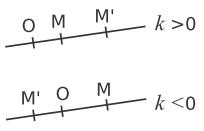
\includegraphics[scale=0.65]{../img/homo_v2}
				\end{center}
			\end{column}
		\end{columns}
		
			
			
	\end{alertblock}
\end{frame}

\begin{frame}
	\frametitle{Homothéties}
	\framesubtitle{}
	
	\begin{block}{Remarque}
		\begin{itemize}
			\item Si $k>1$ ou $k<-1$, \pause la figure est un agrandissement de la figure initiale.\pause
			\item Si $-1<k<0$ ou $0<k<1$,\pause la figure est une réduction de a figure initiale. 
		\end{itemize}
	\end{block}
	
	\begin{block}{Propriétés}
		Par une \homo\ de rapport $k$, l'image :
		\begin{itemize}
			\item d'une droite est une droite qui lui est parallèle;
			\item d'un segment $[MN]$ est un segment $[M'N']$ de longueur $k \times MN$ (si $k>0$) ou $-k \times MN$ (si $k<0$)
		\end{itemize}
	\end{block}
\end{frame}

\section{Théorème de Thalès}

\begin{frame}
	%\frametitle{Théorème de Thalès}

	\begin{alertblock}{Propriété}
		Si deux droites \dte{BM} et \dte{CN} sécantes en $A$ sont coupées par deux droites parallèles \dte{BC} et \dte{MN}, \textbf{alors :}
		
		\begin{equation*}
		\dfrac{A\textcolor{Blue}{M}}{A\textcolor{Red}{B}}=\dfrac{A\textcolor{Blue}{N}}{A\textcolor{Red}{C}}=\dfrac{\textcolor{Blue}{MN}}{\textcolor{Red}{BC}}
		\end{equation*}
	\end{alertblock}
	
	\begin{block}{Configurations de Thalès}
		\begin{columns}
			\begin{column}{3cm}
				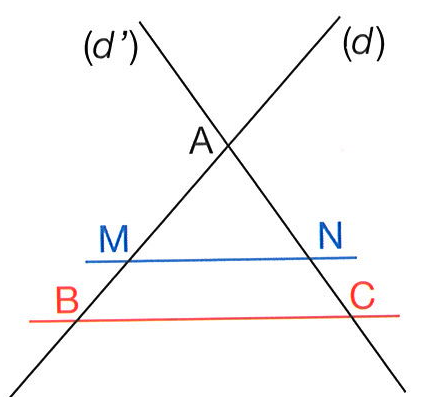
\includegraphics[scale=0.3]{../img/thales3}
			\end{column}
			\begin{column}{3cm}
				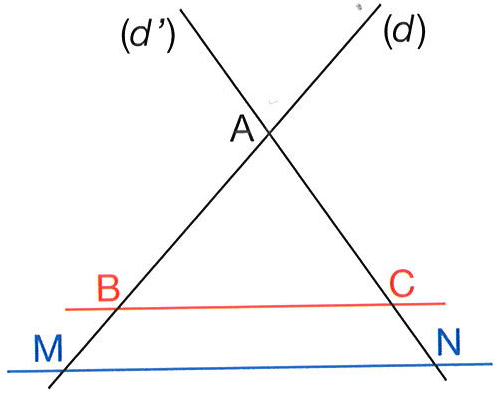
\includegraphics[scale=0.27]{../img/thales2}
			\end{column}
			
			\begin{column}{3cm}
				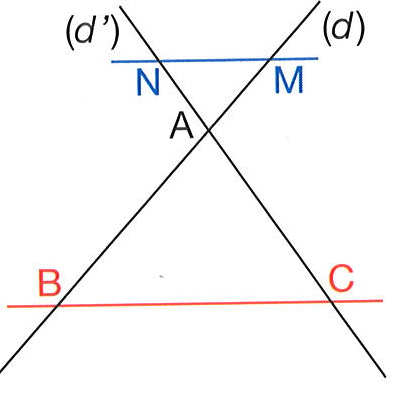
\includegraphics[scale=0.3]{../img/thales1}
			\end{column}
		\end{columns}
		
		Le triangle AMN est l'image du triangle ABC par une \homo\ de centre A.
	\end{block}
\end{frame}


\section{Réciproque du théorème de Thalès}

\end{document}